% !TeX spellcheck = en_US
\section{Problem 15}
\subsection{Question A}
Reducing computing time and resource consumption through efficient techniques is necessary for implementing rapid convolutions in image processing or deep learning activities. Convolution of an image with a $k x k$ kernel is a popular technique. There are quite some techniques to implement it. In this exercise we will examine two of them.\\
One method is to scan horizontally across the source, reading a $k-wide$ strip and computing
the 1-wide output strip one value at a time.\\
Another alternative, possibly more effective approach is to read a $k + \Delta$ wide strip
and compute a $\Delta-wide$ output strip. \\
Due to the fact that it can eliminate pointless calculations, enhance memory access patterns and make better use of hardware acceleration features, this alternative method is frequently chosen. The selection of $\Delta$, however, is crucial since an excessively high value could result in higher memory needs and lower performance gains. Thus, the ideal choice of $\Delta$ strikes a balance between computational effectiveness and memory and hardware limitations.
\\

In more details, this approach is often known as “vectorized convolution” or “strip mining” and it can lead to more efficient convolution operations.

Here are some advantages of the alternative approach and why the latter is preferred:
\begin{itemize}
	\item \underline{Memory Access Pattern}\\
	This approach reads a wider strip of input data, $k+\Delta wide$, all at once, increasing the amount of data reuse. In comparison to reading $k-wide$ strips repeatedly, this can make greater use of memory hierarchy and cache, reducing the amount of memory accesses.
	\item \underline{Parallelization}\\
	The wider strip allows for more opportunities for parallelism since we can perform computations for multiple output values simultaneously. This can be beneficial for optimizing computations on modern hardware, like GPUs or parallel CPU architectures that have vectorized instructions and perform the same operation on multiple data points in parallel. We can make better use of these vectorized processes by computing an $\Delta-wide$ output strip, which will allow you to process several outputs in parallel and greatly improve computational performance.
	\item \underline{Reduced Overhead}\\
	Reading a larger strip of input data with fewer iterations, reduces loop overhead and branching, which can lead to improved performance.
	\item \underline{Input/Output Bandwidth Utilization}\\
	As the overhead of each read operation is reduced, reading data in bigger chunks can make better use of the memory bandwidth.
\end{itemize}

However, there is a limit to how large we should choose the valued of $\Delta$, and it depends on various factors, such as memory constraints, cache size and hardware architecture. By increasing $\Delta$ too much it could lead to increased memory usage and cache trashing, negating the benefits of the approach. Larger $\Delta$ values require more memory to store the wider strips of the input image and intermediate computation results. Moreover, a larger $\Delta$ requires more computation to process the wider strip, which might introduce additional overhead and in the end it may not yield significant performance improvements.\\

Everything considered, finding a balance between the advantages of more parallelism and data reuse and the possible disadvantages of more memory and processing is crucial. We could find the best option for the value of $\Delta$ by profiling and experimenting with various values on the particular hardware we are targeting. In practice, finding the ideal $\Delta$ often involves empirical testing and optimization based on the specific application and hardware configuration. \\

Overall, the alternative approach of reading a $k + \Delta$ wide strip and computing a $\Delta-wide$ output strip is preferable due to improved memory access patterns, increased parallelism, and reduced overhead. However, the choice of $\Delta$ should be carefully considered based on hardware limitations and performance trade-offs.
\vspace{3mm}

\subsection{Question B}
We will attempt to apply and test these two approaches in relation to one another. For this reason, we will construct a random sample image of size $228 x 228$. A sequence of random $3x3$, $7x7$, and $11x11$ kernels will then convolve with this image. We can have a better understanding of the two options and the reasons for the preference for the second one by comparing their execution times.\\

We will extract our results from the \textit{"sample\_times.py"} code.

\begin{figure}[h]
	\centering
	\begin{subfigure}{0.45\linewidth}
		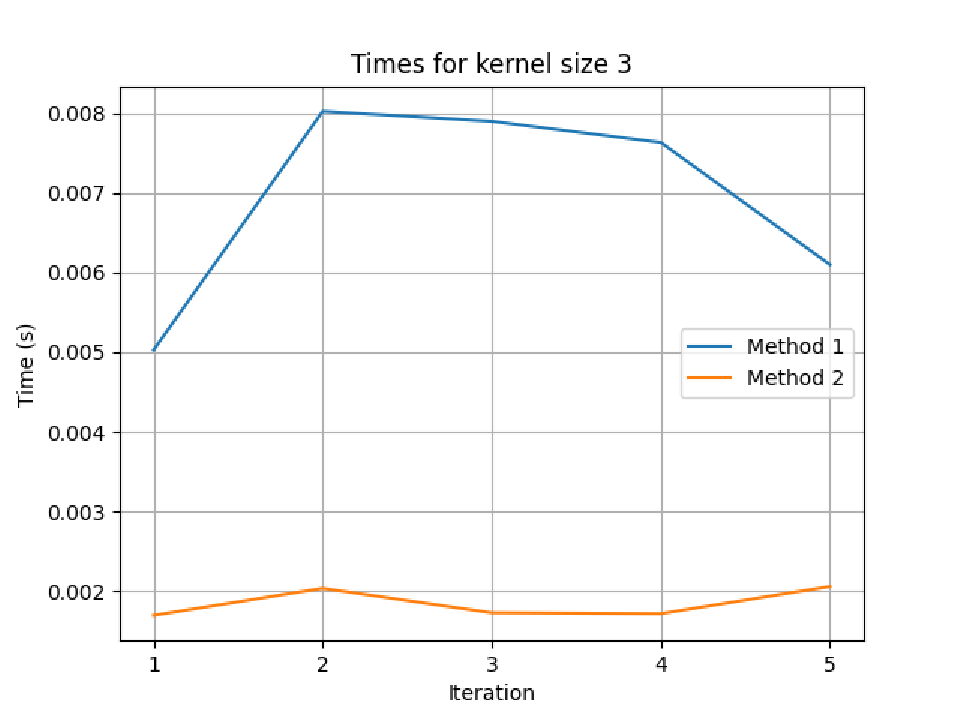
\includegraphics[width=\linewidth]{../Problem 15/figure_kernel3.pdf}
		\caption{Plot for $3x3$ kernel}
		\label{fig:sample_kernel3}
	\end{subfigure}
	\begin{subfigure}{0.45\linewidth}
		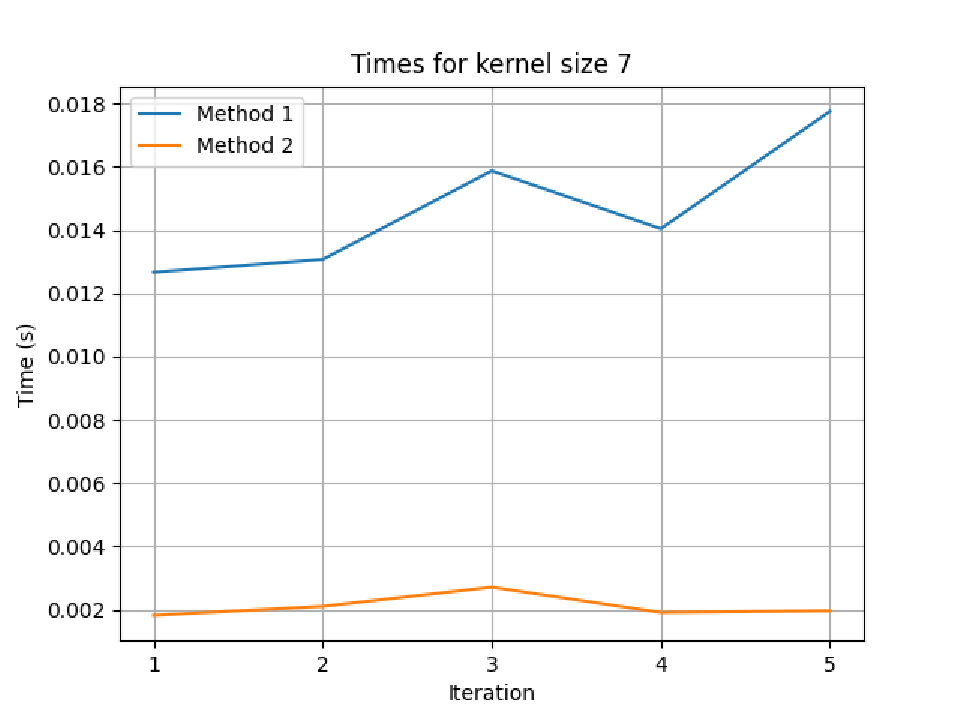
\includegraphics[width=\linewidth]{../Problem 15/figure_kernel7.pdf}
		\caption{Plot for $7x7$ kernel}
		\label{fig:sample_kernel7}
	\end{subfigure}
	\begin{subfigure}{0.45\linewidth}
		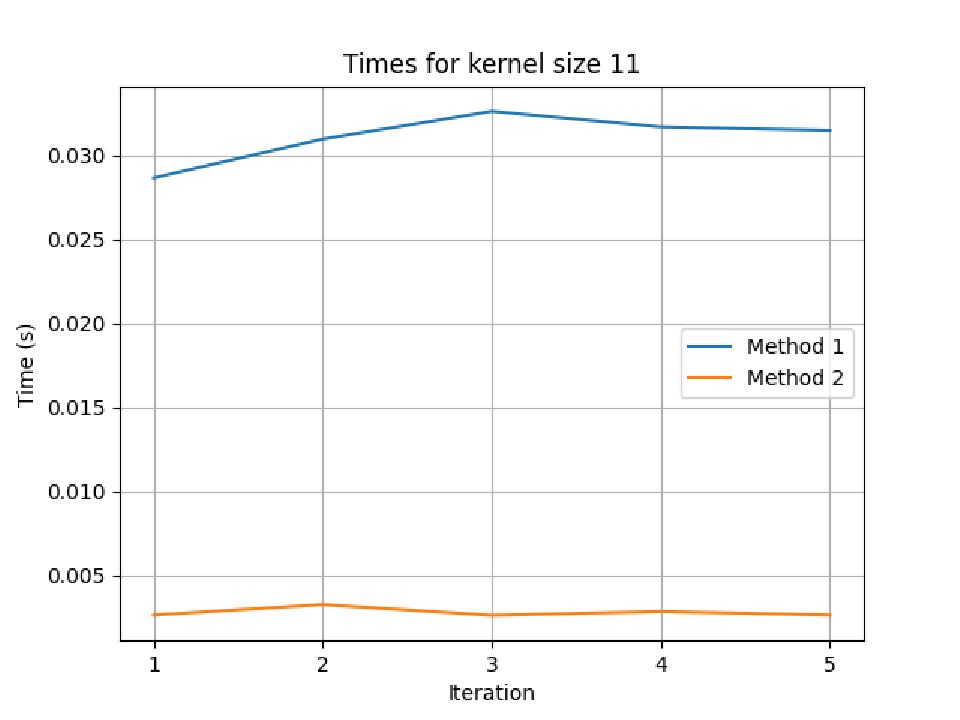
\includegraphics[width=\linewidth]{../Problem 15/figure_kernel11.pdf}
		\caption{Plot for $11x11$ kernel}
		\label{fig:sample_karnel11}
	\end{subfigure}
	%\caption{Plots for }
\end{figure}

The provided plots offer a visual representation of the performance metrics for each method,allowing us to discern patterns and draw conclusions. With these visual data points we will analyze with more details the execution times.\\

\textbf{For 3x3 kernel}
\begin{itemize}
		\item \underline{Method 1}: The execution times start relatively high and show a notable peak at iteration two. This could indicate that for small kernel sizes, the method's overhead associated with reading data and computing the output sequentially impacts performance negatively. This peak may suggest a temporary computational load or caching issue that affected the performance at this specific point. Following the peak, there is a slight reduction in the execution time for subsequent iterations, which could indicate some level of caching benefit as the computation progresses.
		\item \underline{Method 2}: The consistent low execution times suggest that reading a $k+\Delta$ wide strip and computing a $\Delta-wide$ output is significantly more efficient. The method likely benefits from increased data locality, allowing for better utilization of cache hierarchies and minimizing the number of memory accesses required. It shows a remarkably consistent execution time across all iterations, reinforcing its efficient use of resources and possibly better memory access patterns.
\end{itemize}

\textbf{For 7x7 kernel}	
\begin{itemize}
		\item \underline{Method 1}: As the kernel size increases, the execution times for Method 1 also rise. There is a steady increase in execution time from the first to the fifth iteration, with the peak occurring at the fifth iteration and continuing increasing.  This pattern implies that the performance of the approach deteriorates with increasing kernel size, most likely because of higher computational load and more frequent memory access conflicts.
		\item \underline{Method 2}: Remarkably, this method shows an incremental rise in execution time but remains substantially faster that Method 1. It maintains a remarkably consistent and low execution time throughout all iterations. This resilience to increased kernel size suggests that Method 2 efficiently manages the additional computational complexity, potentially through better parallelization, without significant impact on performance..
\end{itemize}

\textbf{For 11x11 kernel}
\begin{itemize}
	\item \underline{Method 1}: The continued upward pattern in execution time for larger kernels confirms the method's limited scalability. Method 1 starts with a higher execution time in the first iteration, which then remains relatively flat for subsequent iterations. The significant increase from 7x7 to 11x11 kernels suggests that the method may be approaching a computational bottleneck, possibly due to an exponential increase in the number of operations required.
	\item \underline{Method 2}: Even at this larger kernel size, Method 2's execution time increases only slightly, maintaining a considerable lead over Method 1. Method 2 exhibits a very stable and low execution time across all five iterations, with no noticeable increase or decrease. This indicates a near-linear scalability, likely due to the method's effective amortization of the computational and memory access costs over a larger output strip.
\end{itemize}		

The major differences in efficiency and scalability between the two approaches are made clear by this in-depth examination of the supplied charts. For the purpose of this exercise and in general for computational neural networks and image processing we can truly understand why Method 2 is the better choice. It is due to its consistent and better performance at all kernel sizes, its stability and low execution time at all costs. Last but not least, Method 2 can be considered more memory friendly, as it likely reduces memory bandwidth requirements and cache thrashing compared to Method 1. The consistent execution times of Method 2 across various kernel sizes support the notion of its efficient memory usage.
	







